\documentclass[ukenglish]{beamer}

%%% Dichiarazione dei pacchetti standard.
\usepackage[utf8x]{inputenc}
\usepackage{graphicx}    % inclusione graph images (eps)
\usepackage{units}
\usepackage{url}
\usepackage{lmodern}
\usepackage[T1]{fontenc}
%gets rid of bottom navigation bars

\usetheme{Boadilla}
\usecolortheme{wolverine}

\setbeamertemplate{footline}[frame number]{}
%\setbeamertemplate{navigation symbols}{\insertframenumber} 
\setbeamertemplate{navigation symbols}{} 
\graphicspath{{./images/}}
    
%%% Titolo e autore.
\title[Top Partners at the LHC]{A search for new physics at the LHC:\\
top partners into same-sign leptons.}
\author{Matteo Abis\\
\url{matteo.abis@cern.ch}}
\institute{Università di Padova and CERN}
\date{\today}

\begin{document}
\begin{frame}
  \titlepage
\end{frame}
 
\begin{frame}
    \frametitle{Physics beyond the Standard Model}
    \begin{itemize}
        \item What is the Standard Model of particle physics?
        \item Why do physicists like it?
        \item Why are we not completely satisfied with it?
    \end{itemize}
\end{frame}

\begin{frame}
    \frametitle{Modern physics and the Standard Model}
    \begin{block}
        {Simmetry}
        Let's review it in ``old'' physics first.
    \end{block}
\end{frame}

\begin{frame}
    \frametitle{What was ``old'' physics like?}
    \begin{enumerate}
        \item 
    Theory $+$ experiment $\longrightarrow$ force or potential energy.
    %[$\vec{F} = -\vec{\nabla}U(x)$]
\item potential $\rightarrow$ simmetries $\rightarrow$ simple equations
    $\rightarrow$ happy physicists!
    \end{enumerate}
    \uncover<2->{
    \begin{block}
        {Gravity}
        \begin{figure}[h!]
            \centering
                $\vcenter{\hbox{
                    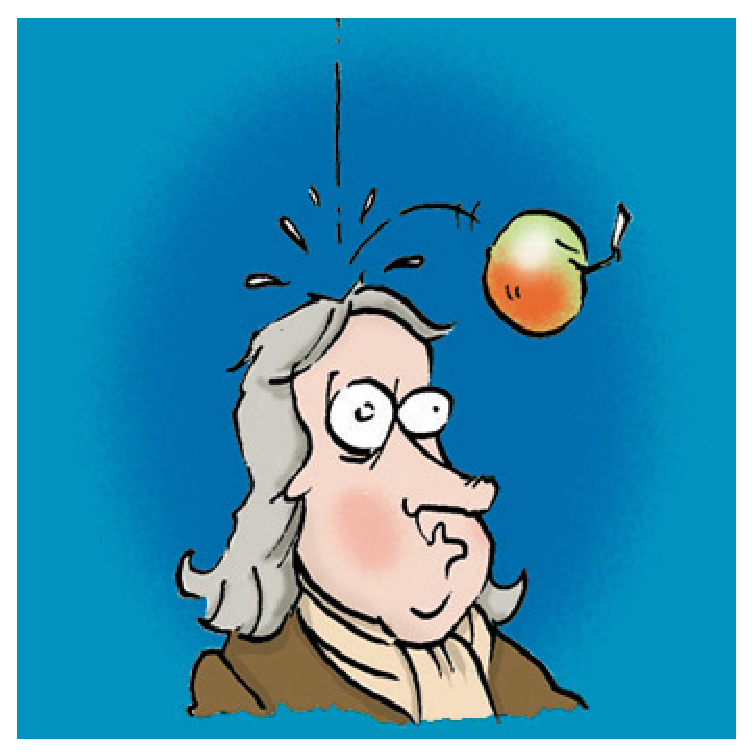
\includegraphics[height=.2\textheight]{newton}}} + 
                \vcenter{\hbox{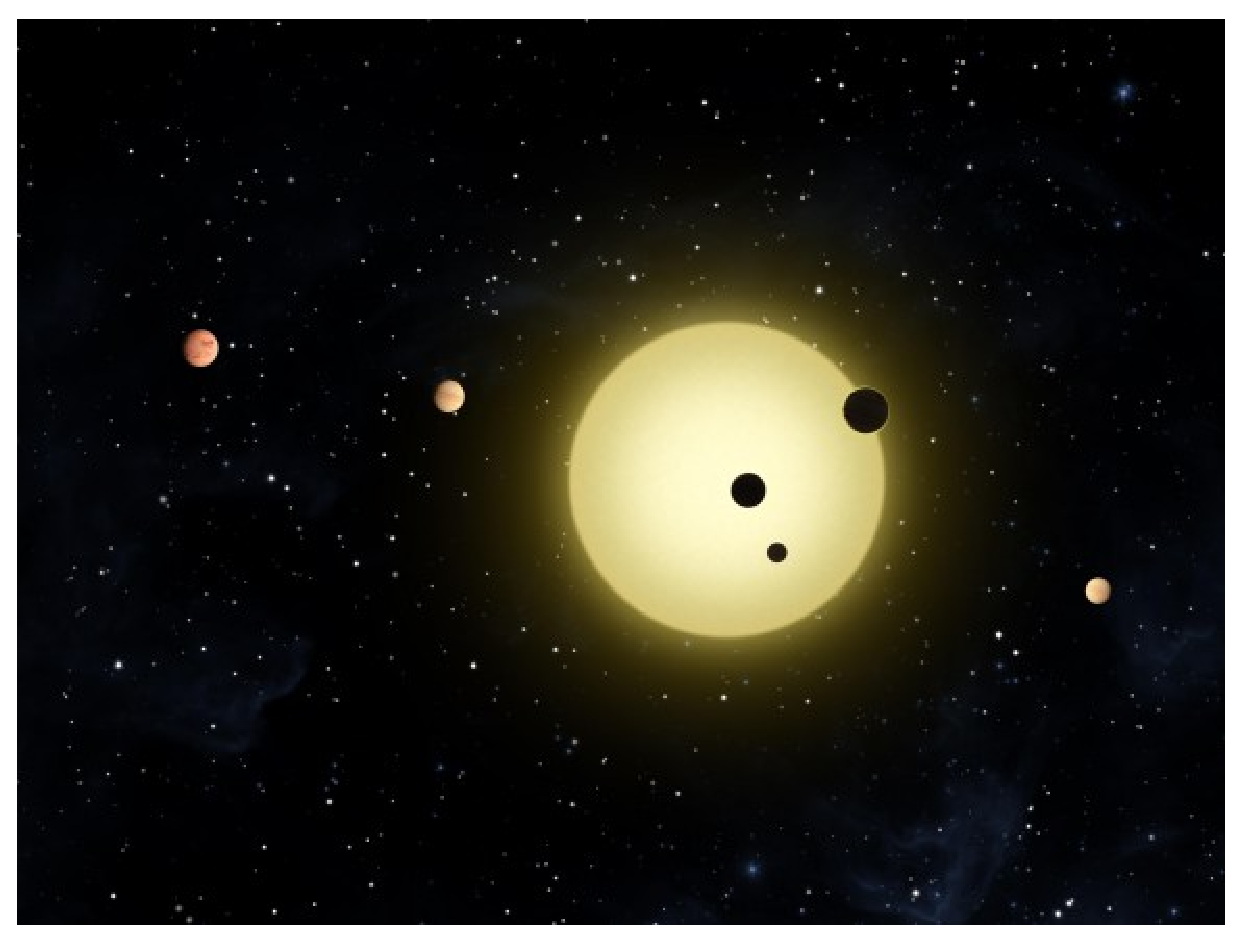
\includegraphics[height=.2\textheight]{kepler}}}$
        $\longrightarrow U(r) = -\frac{GMm}{r}$.
        \end{figure}

        \uncover<3->{
            Depends only on the distance $r$, simmetry under rotations.

            Angular momentum is constant.

            Easy equation, the orbits are ellipses.
        }
    \end{block}
}
\end{frame}

\begin{frame}
    \frametitle{Simmetries and modern physics}
    \framesubtitle{A first success: the birth of special relativity}
    \centering
                $\vcenter{\hbox{
                    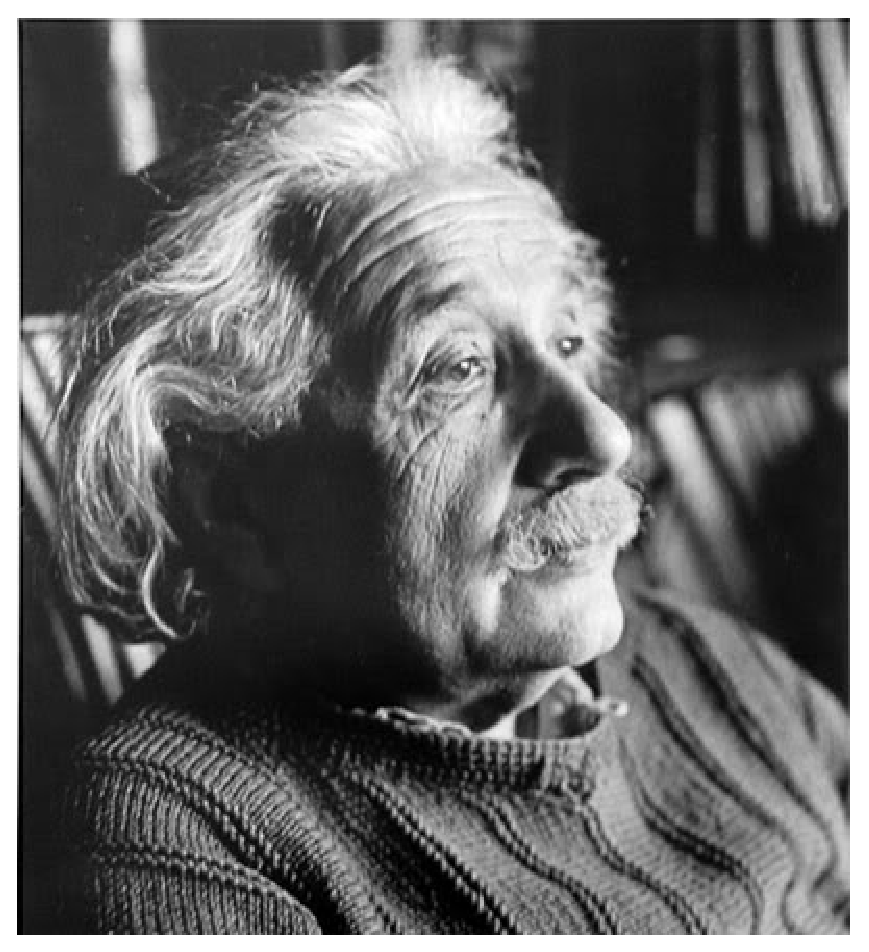
\includegraphics[height=.2\textheight]{einstein}}}$
                    \parbox{.5\textwidth}{
                    Look! Your equations have more\\simmetries than
                we expected!}
                $\vcenter{\hbox{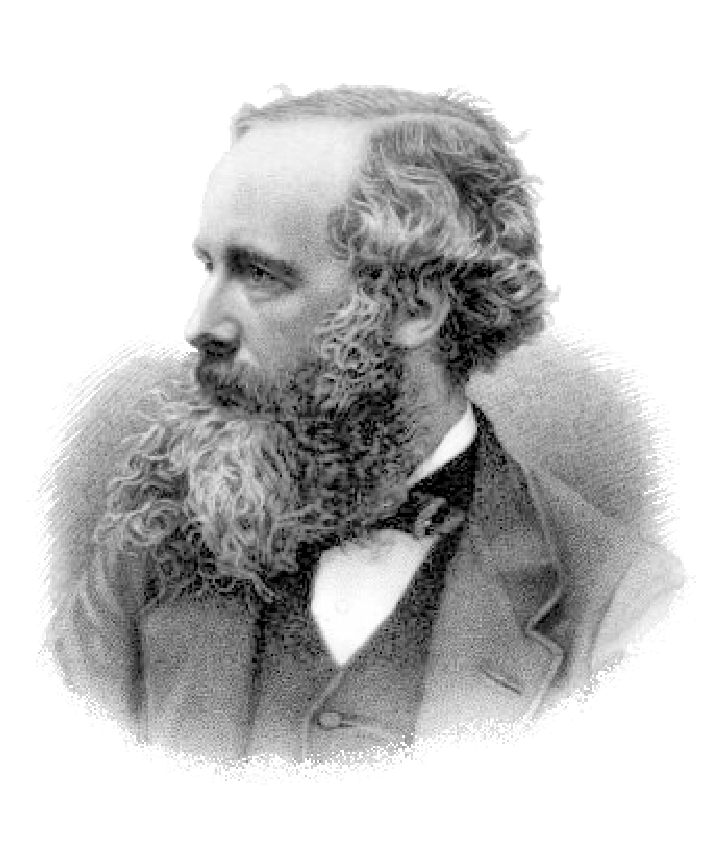
\includegraphics[height=.2\textheight]{maxwell}}}$

                \begin{align*}
                    \nabla \cdot \vec{E} &= \rho\\
                    \nabla \times \vec{B} &= \dfrac{\partial
                        \vec{E}}{\partial t} + \vec{J}\\
                        \cdots
                \end{align*}

                \uncover<2->{
                    \begin{block}{Lorentz transformations}
                        \begin{itemize}
                            \item space and time translations;
                            \item space rotations;
                            \item Lorentz boosts: $t^{'} = \dfrac{t -
                                vx/c^2}{\sqrt{1 - v^2/c^2}}$.
                        \end{itemize}
                 \end{block}}
\end{frame}

\begin{frame}
    \frametitle{Simmetries first!}
    \begin{itemize}
        \item Space and time are homogeneous: no privileged points.
        \item Space is isotropic: no privileged direction.
    \end{itemize}

    What is the most general physical theory compatible with these requirements?

    \uncover<2->{
        \begin{center}
        \alert{Relativistic mechanics!}
\begin{equation*}
        E = mc^2
\end{equation*}
        \end{center}
    Unification of mechanics and electromagnetism, under the
    same simmetry principle.
}
\end{frame}

\begin{frame}
    \frametitle{The Standard Model of particle physics}
    \begin{block}
        {Goal}
    Unification and full description of electromagnetic, weak nuclear force, and strong nuclear
    force.
    \end{block}
    \begin{enumerate}
        \uncover<1-> {\item symmetry principle. [$SU(3) \times SU(2) \times
            U(1)$ invariance]; }
        \uncover<2->{\item particles: what is the universe made of?}
    \end{enumerate}

    \begin{figure}[h!]
        \centering
        \only<3>{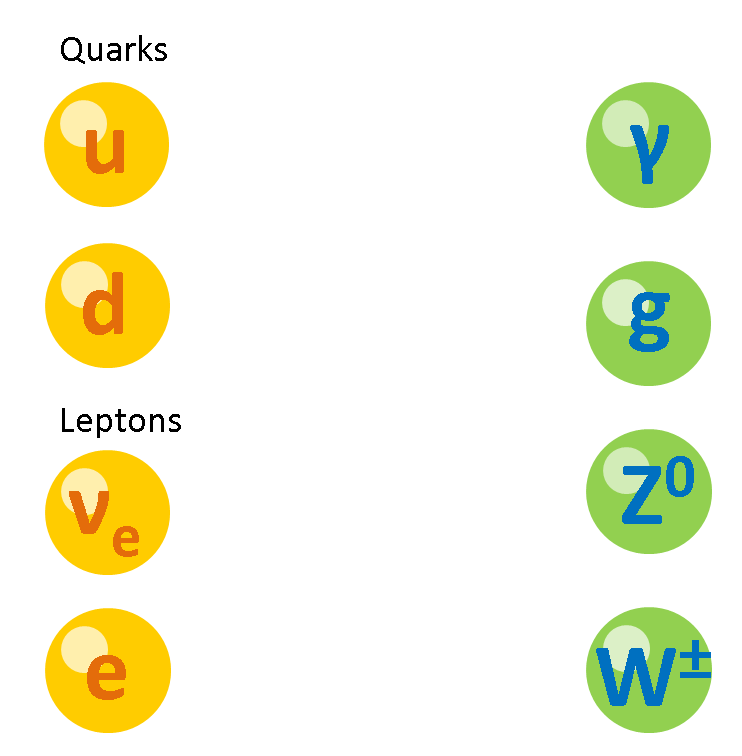
\includegraphics[width=.35\textwidth]{standard_model_particles_1family}}
        \only<4>{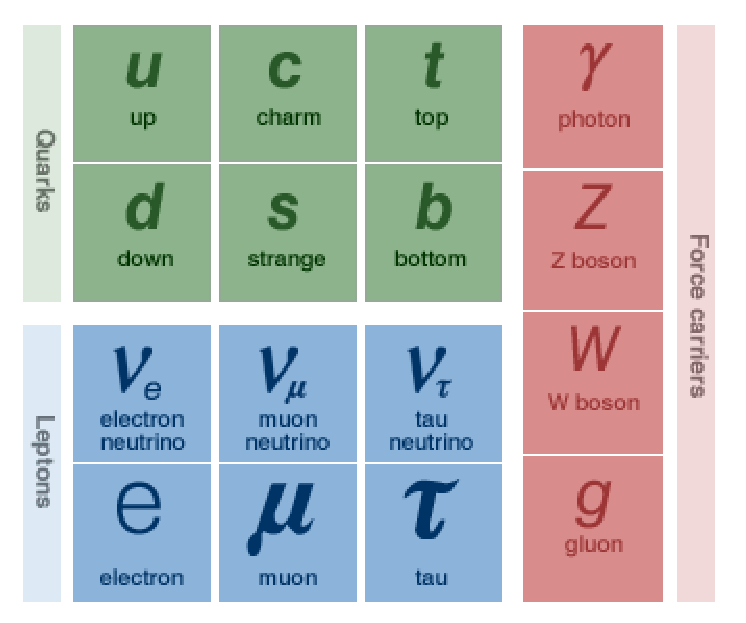
\includegraphics[width=.35\textwidth]{standard_model_particles}}
    \end{figure}
\end{frame}

\begin{frame}
    \frametitle{Why do physicists like the Standard Model?}
    \begin{block}
        {Theory}
        Very few and simple premises, simmetry principles. Unbelievable
        predicting power for all kind of phenomena.
    \end{block}
    \begin{block}
        {Experiment}
        \begin{align*}
    g_{\text{exp}}/2 &= 1.001\,159\,652\,180\,85(76)\\
    g_{\text{th}}/2 &= 1.001\,159\,652\,177\,60(520)
        \end{align*}
        \begin{itemize}
            \item Incredible experimental precision: less than one part per
                trillion.
            \item Unmatched agreement between theory and experiment.
        \end{itemize}
    \end{block}
\end{frame}

\begin{frame}
    \frametitle{The Large Hadron Collider}
    \begin{block}
        {$pp$ collisions}
    The ultimate test for the Standard Model.
    \end{block}
    \begin{figure}[h!]
        \centering
        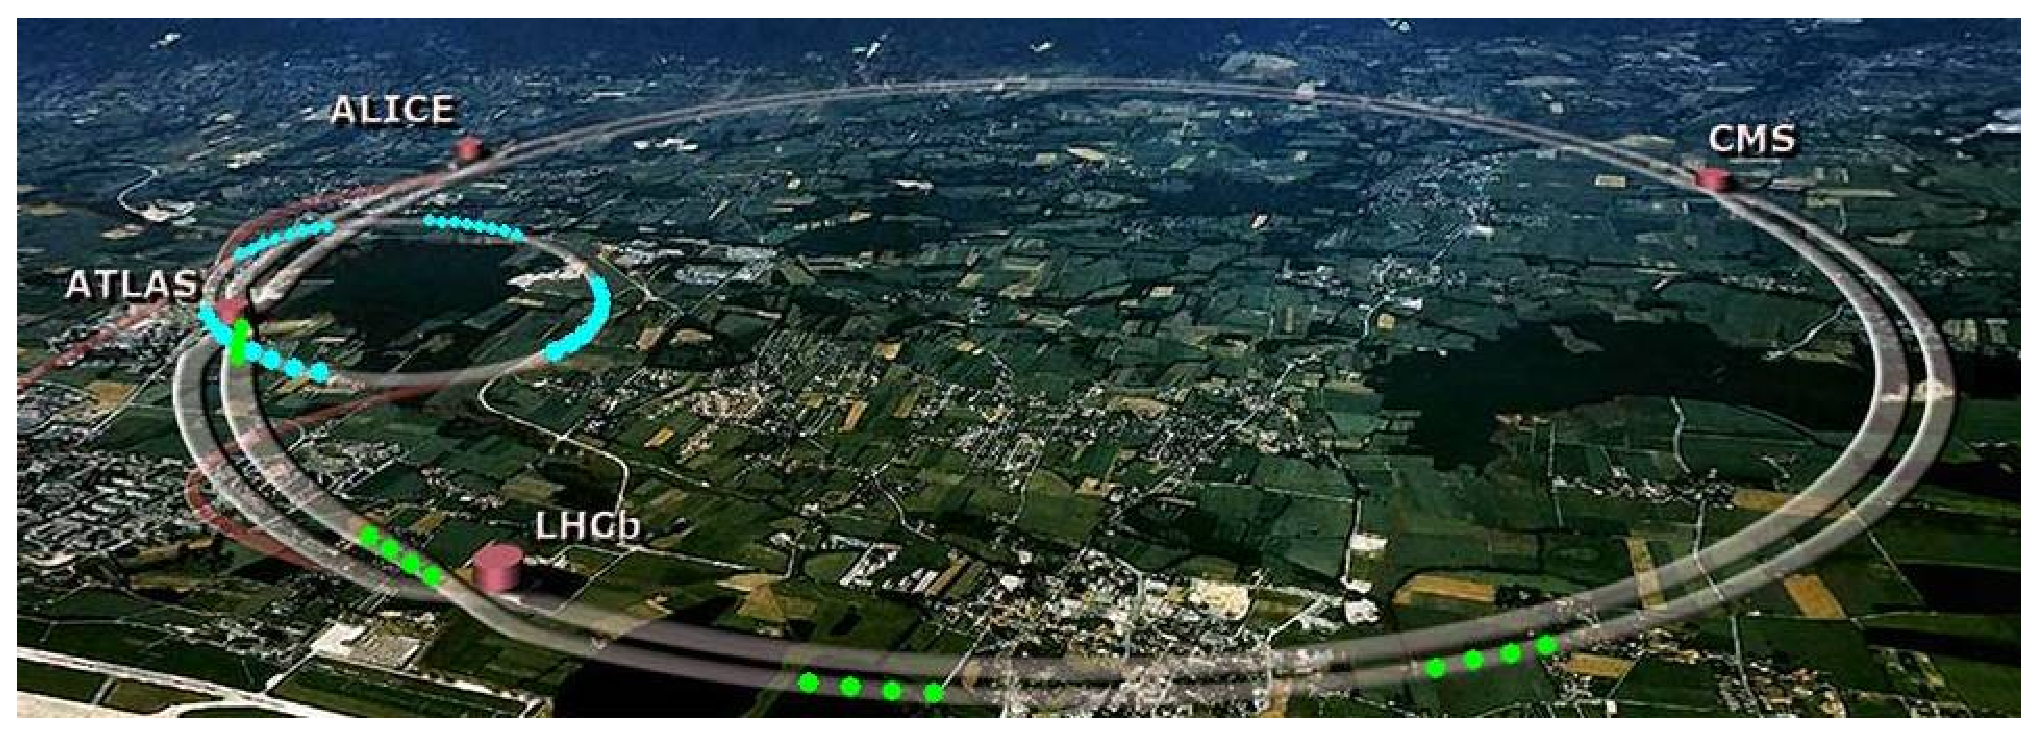
\includegraphics[width=.9\textwidth]{lhc}
    \end{figure}
\end{frame}

\begin{frame}
    \frametitle{The Compact Muon Solenoid}
    \framesubtitle{Also known as the CMS detector}
    \begin{figure}[h]
        \centering
            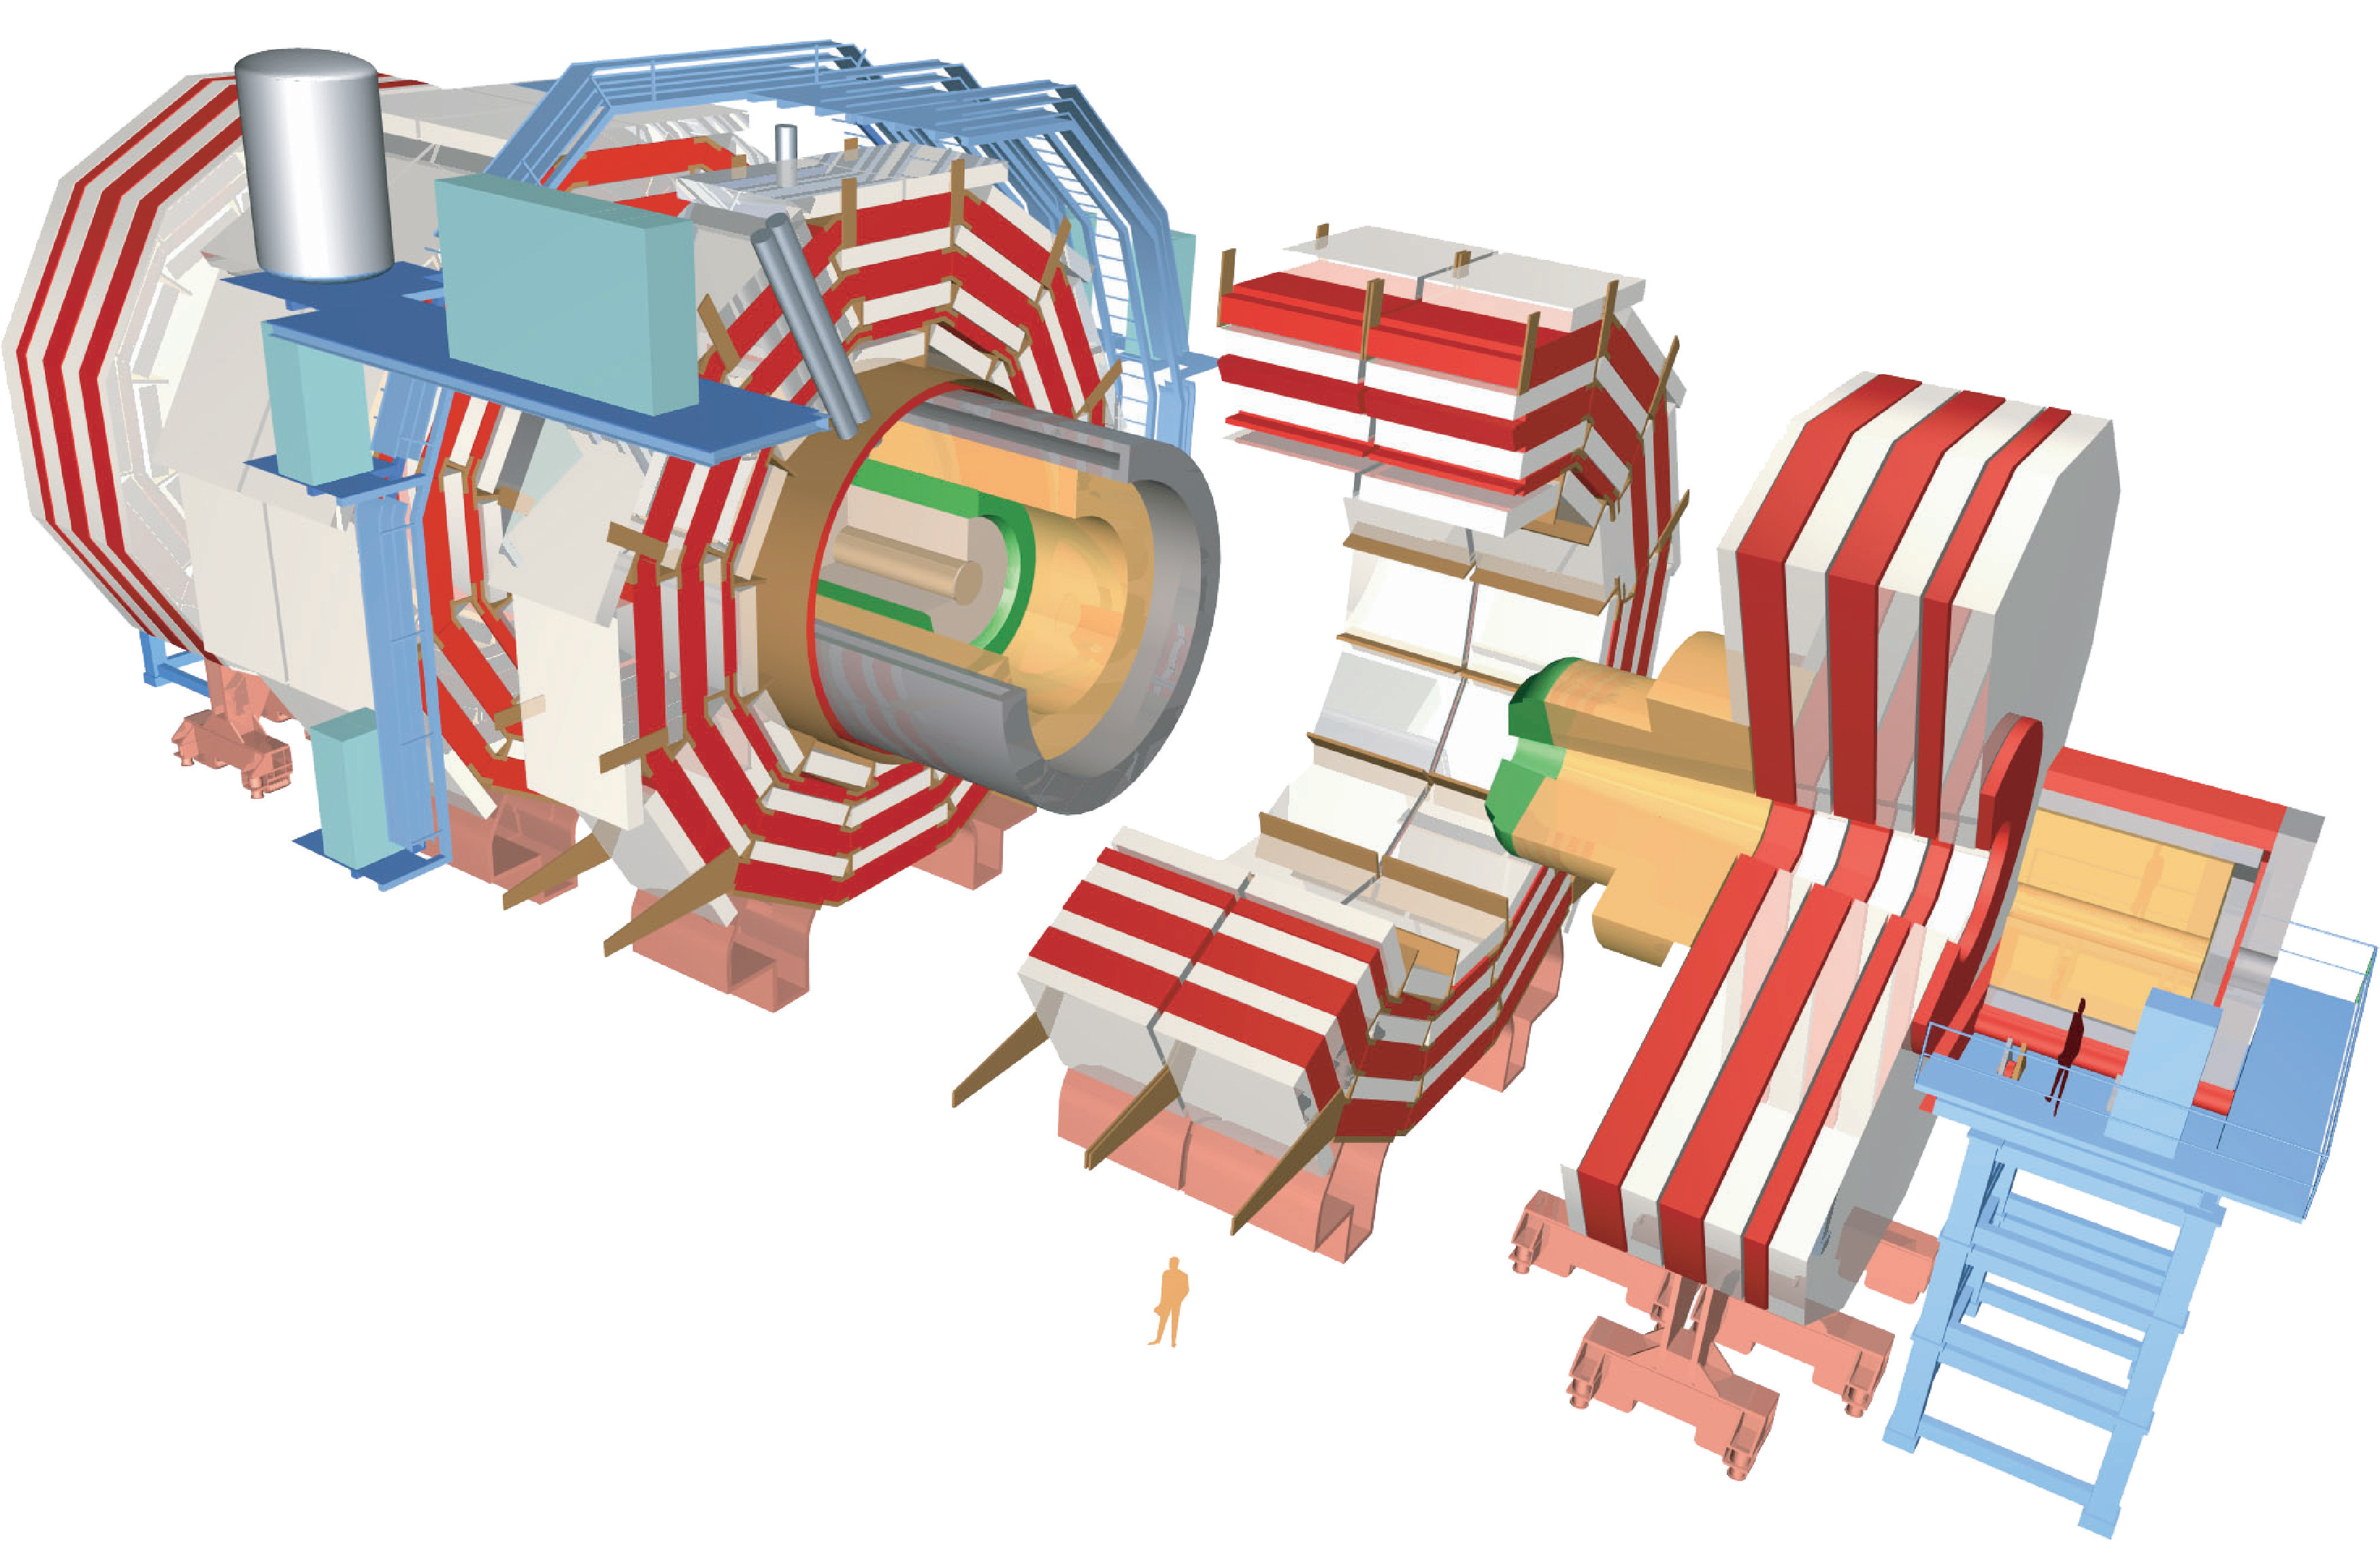
\includegraphics[width=.7\textwidth]{Schematic}
    \end{figure}
    \begin{description}
        \item[Tracker] silicon detectors for the particle momentum;
        \item[Calorimeters] scintillators for the energy;
        \item[$\mu$ detectors] only muons get this far.
    \end{description}
\end{frame}

\begin{frame}
    \frametitle{Shortcomings of the Standard Model}
    \framesubtitle{The hierarchy problem}
    \begin{figure}[h!]
        \centering
        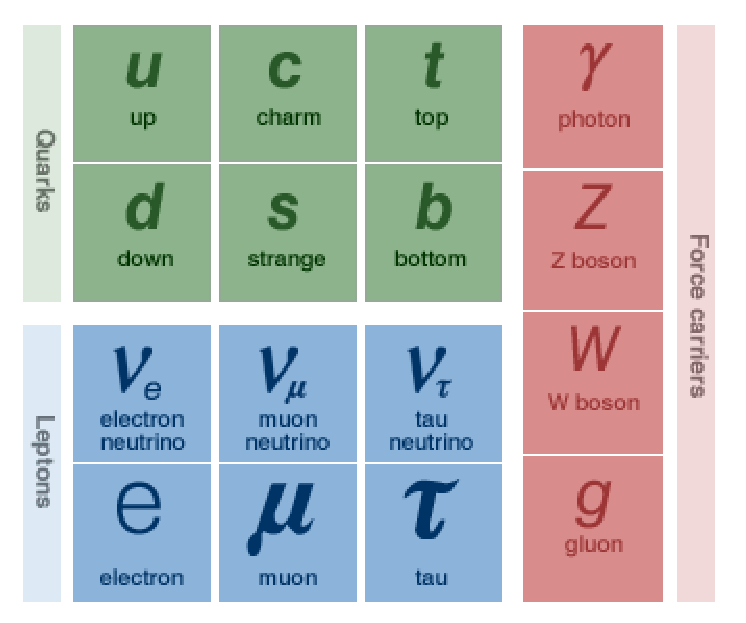
\includegraphics[width=.35\textwidth]{standard_model_particles}
    \end{figure}
    \begin{itemize}
        \item Why three generations?
        \item Why this enormous mass difference?
    \end{itemize}
    \begin{block}
        {Nature for the physicist}
        Beauty $\rightarrow$ similar masses. They now span five orders of magnitude!
    \end{block}
\end{frame}

\begin{frame}
    \frametitle{Top partners}
    \framesubtitle{Extending the Standard Model}

    \begin{block}
        {Common prediction}
        New, unknown particles giving part of their mass to the heavy
        quarks.
    \end{block}
    Large masses for a good reason $\longrightarrow$ happy physicists!
\end{frame}

\begin{frame}
    \frametitle{The hunt for the top partners}
    \framesubtitle{We are looking for their murder scene signature}
    \begin{block}
        {Decay products}
        \begin{itemize}
            \item two same-sign electrons or muons;
            \item many \emph{jets} (at least four);
            \item large mass $\rightarrow$ large energy.
        \end{itemize}
    \end{block}
    \begin{figure}[h]
        \centering
            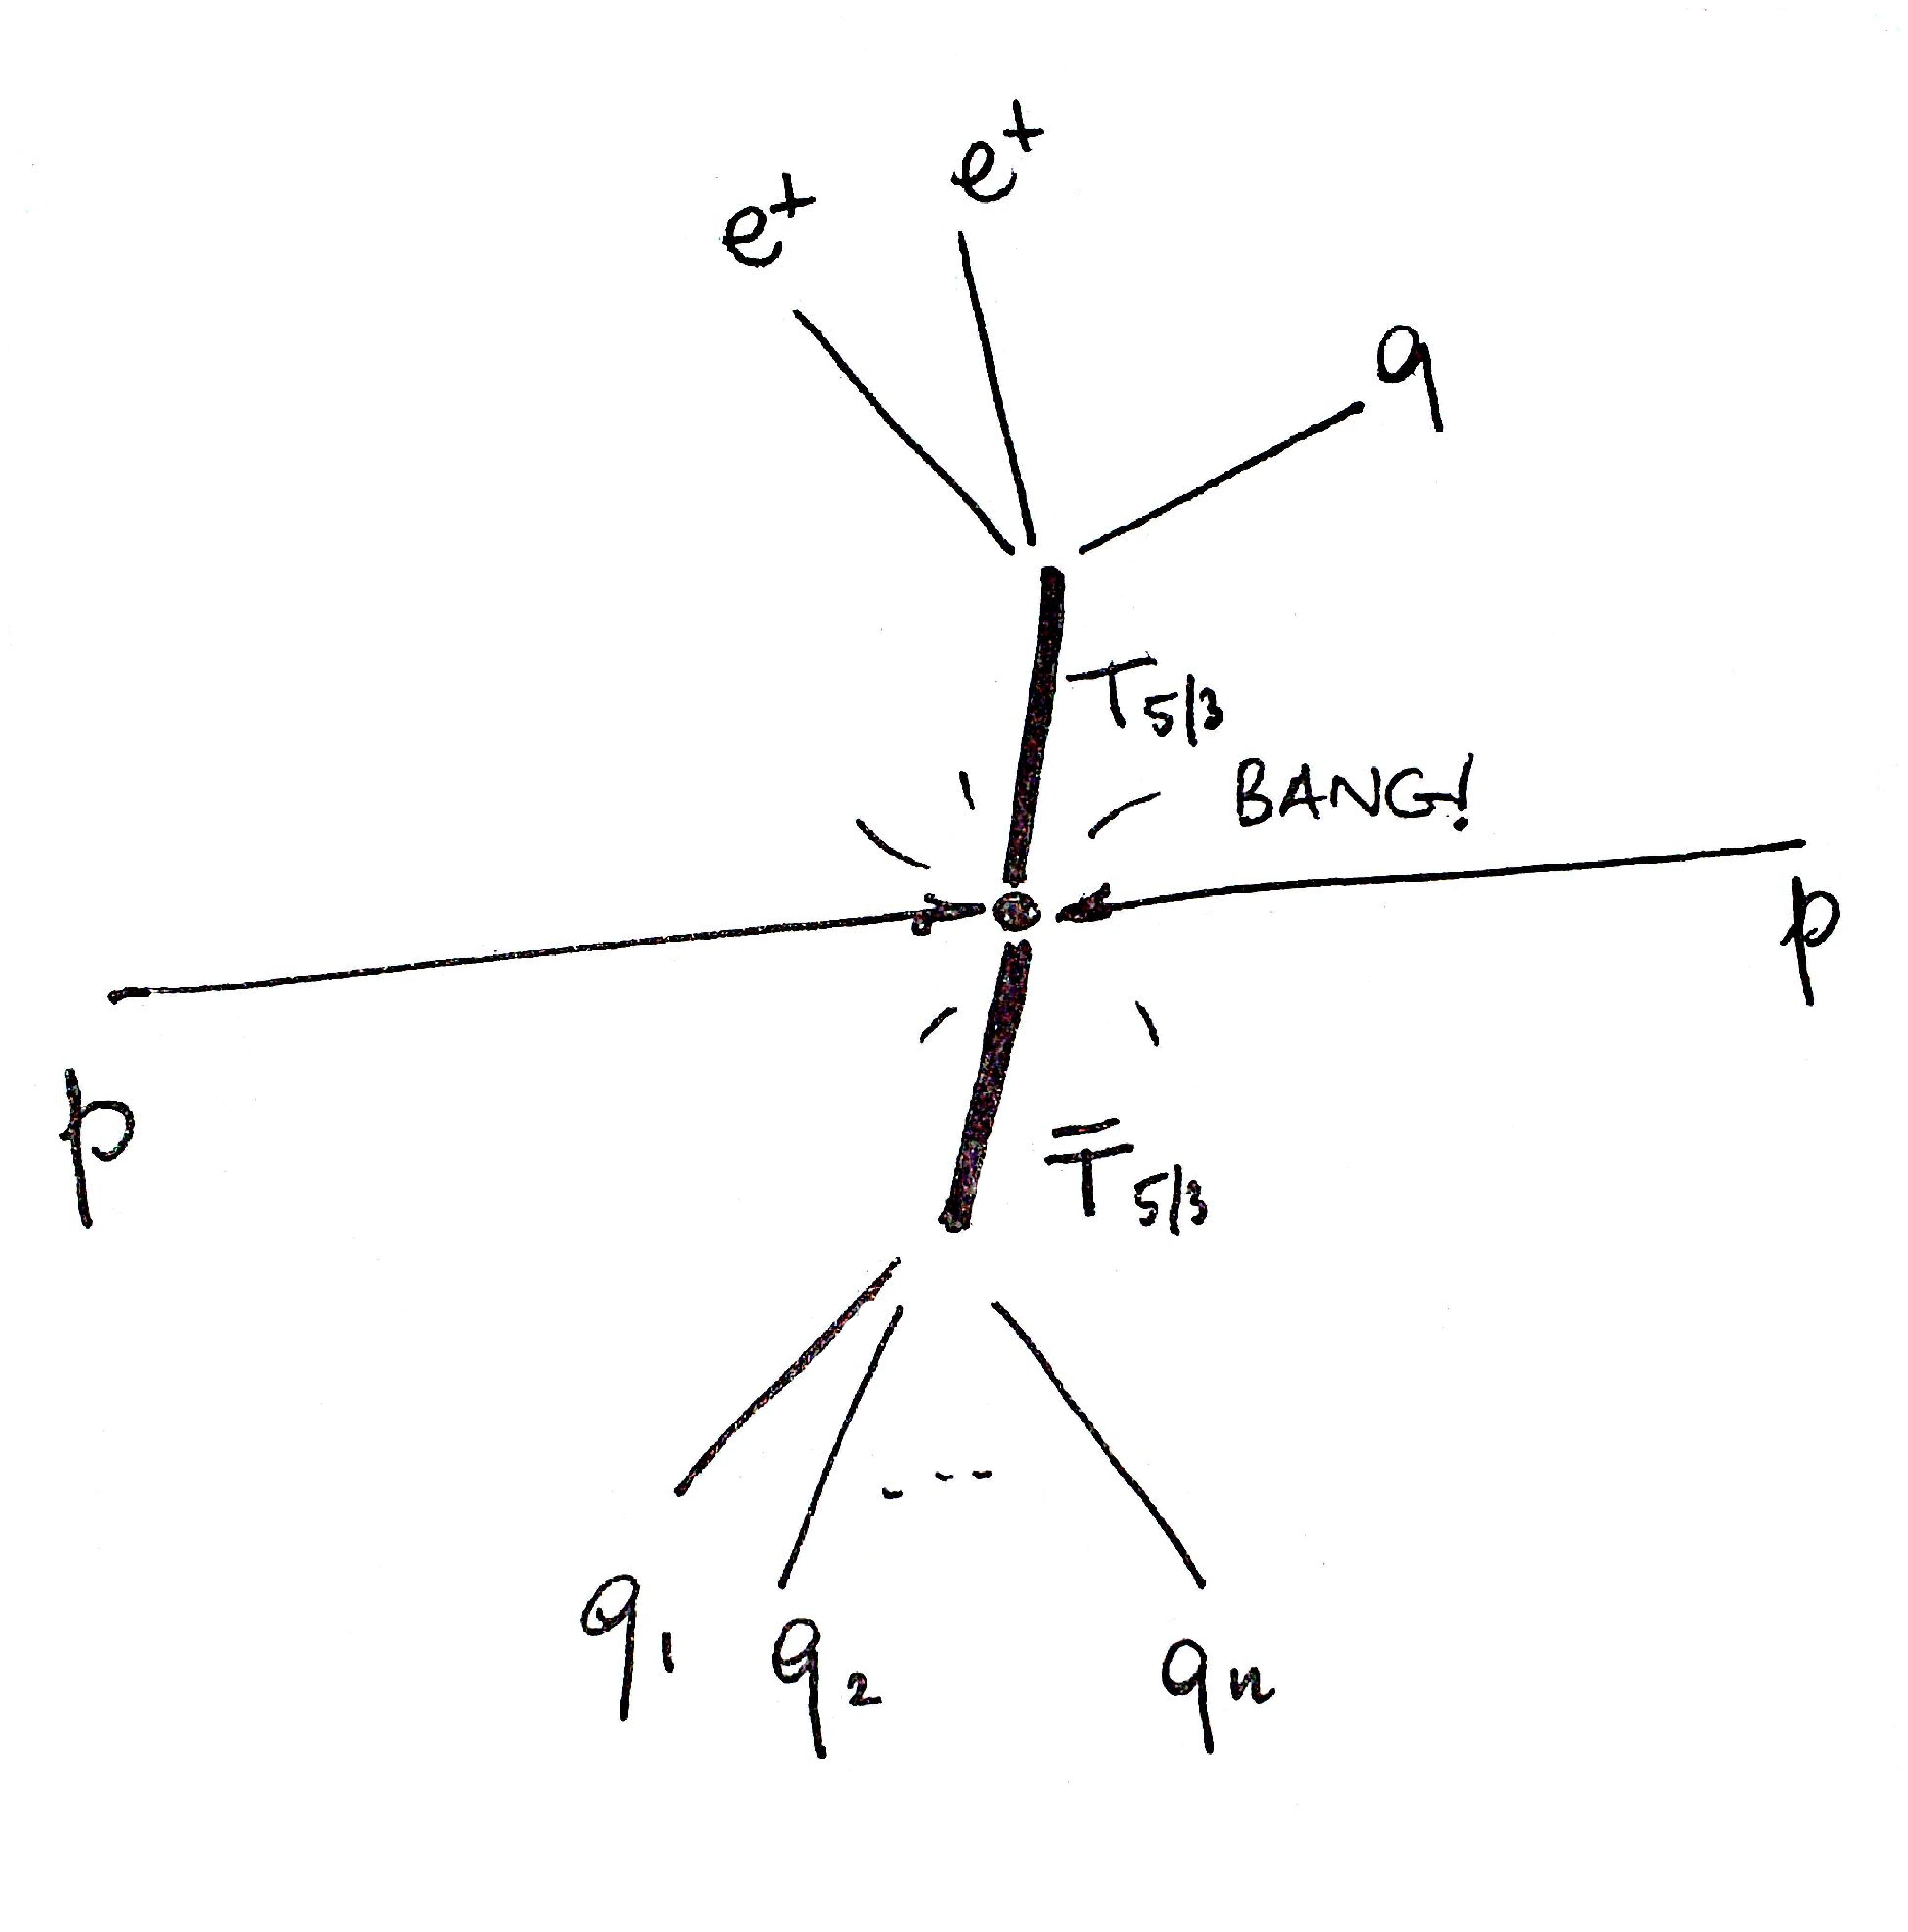
\includegraphics[width=.4\textwidth]{toppartner_decay}
    \end{figure}
\end{frame}

\begin{frame}
    \frametitle{Quarks and jets}
    \framesubtitle{The strong nuclear force and quark confinement}
\begin{block}
    {Jet}
    A group of particles moving in the same direction.\\
    It is the result of the production of quarks.
\end{block}
\uncover<2->{
    \begin{figure}[h]
        \centering
            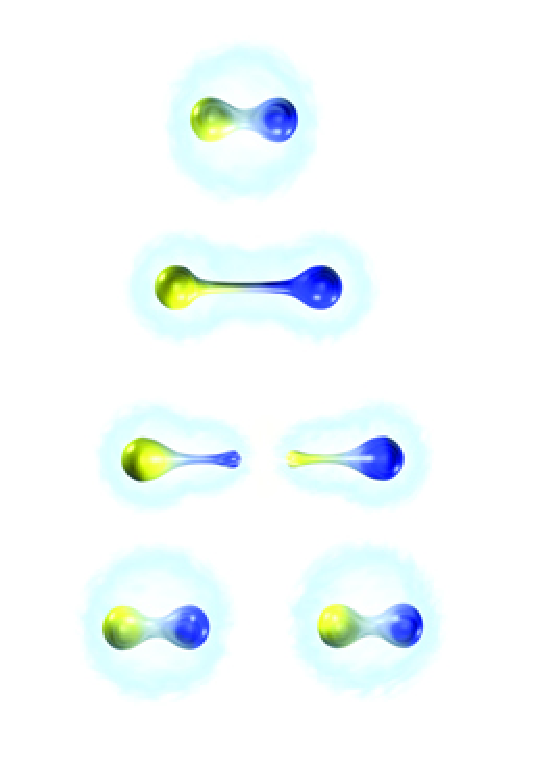
\includegraphics[height=.35\textheight]{quark_confinement}
    \end{figure}
    \begin{itemize}
        \item Force increasing with distance between quarks. Like a spring.
        \item When energy of the spring $> mc^2$ a new quark is created.
        \item Quarks are confined in particles with zero net strong charge.
    \end{itemize}
}
\end{frame}

\begin{frame}
    \frametitle{Quarks and jets}
    \framesubtitle{What you see in the detector}
    \begin{figure}[h]
        \centering
            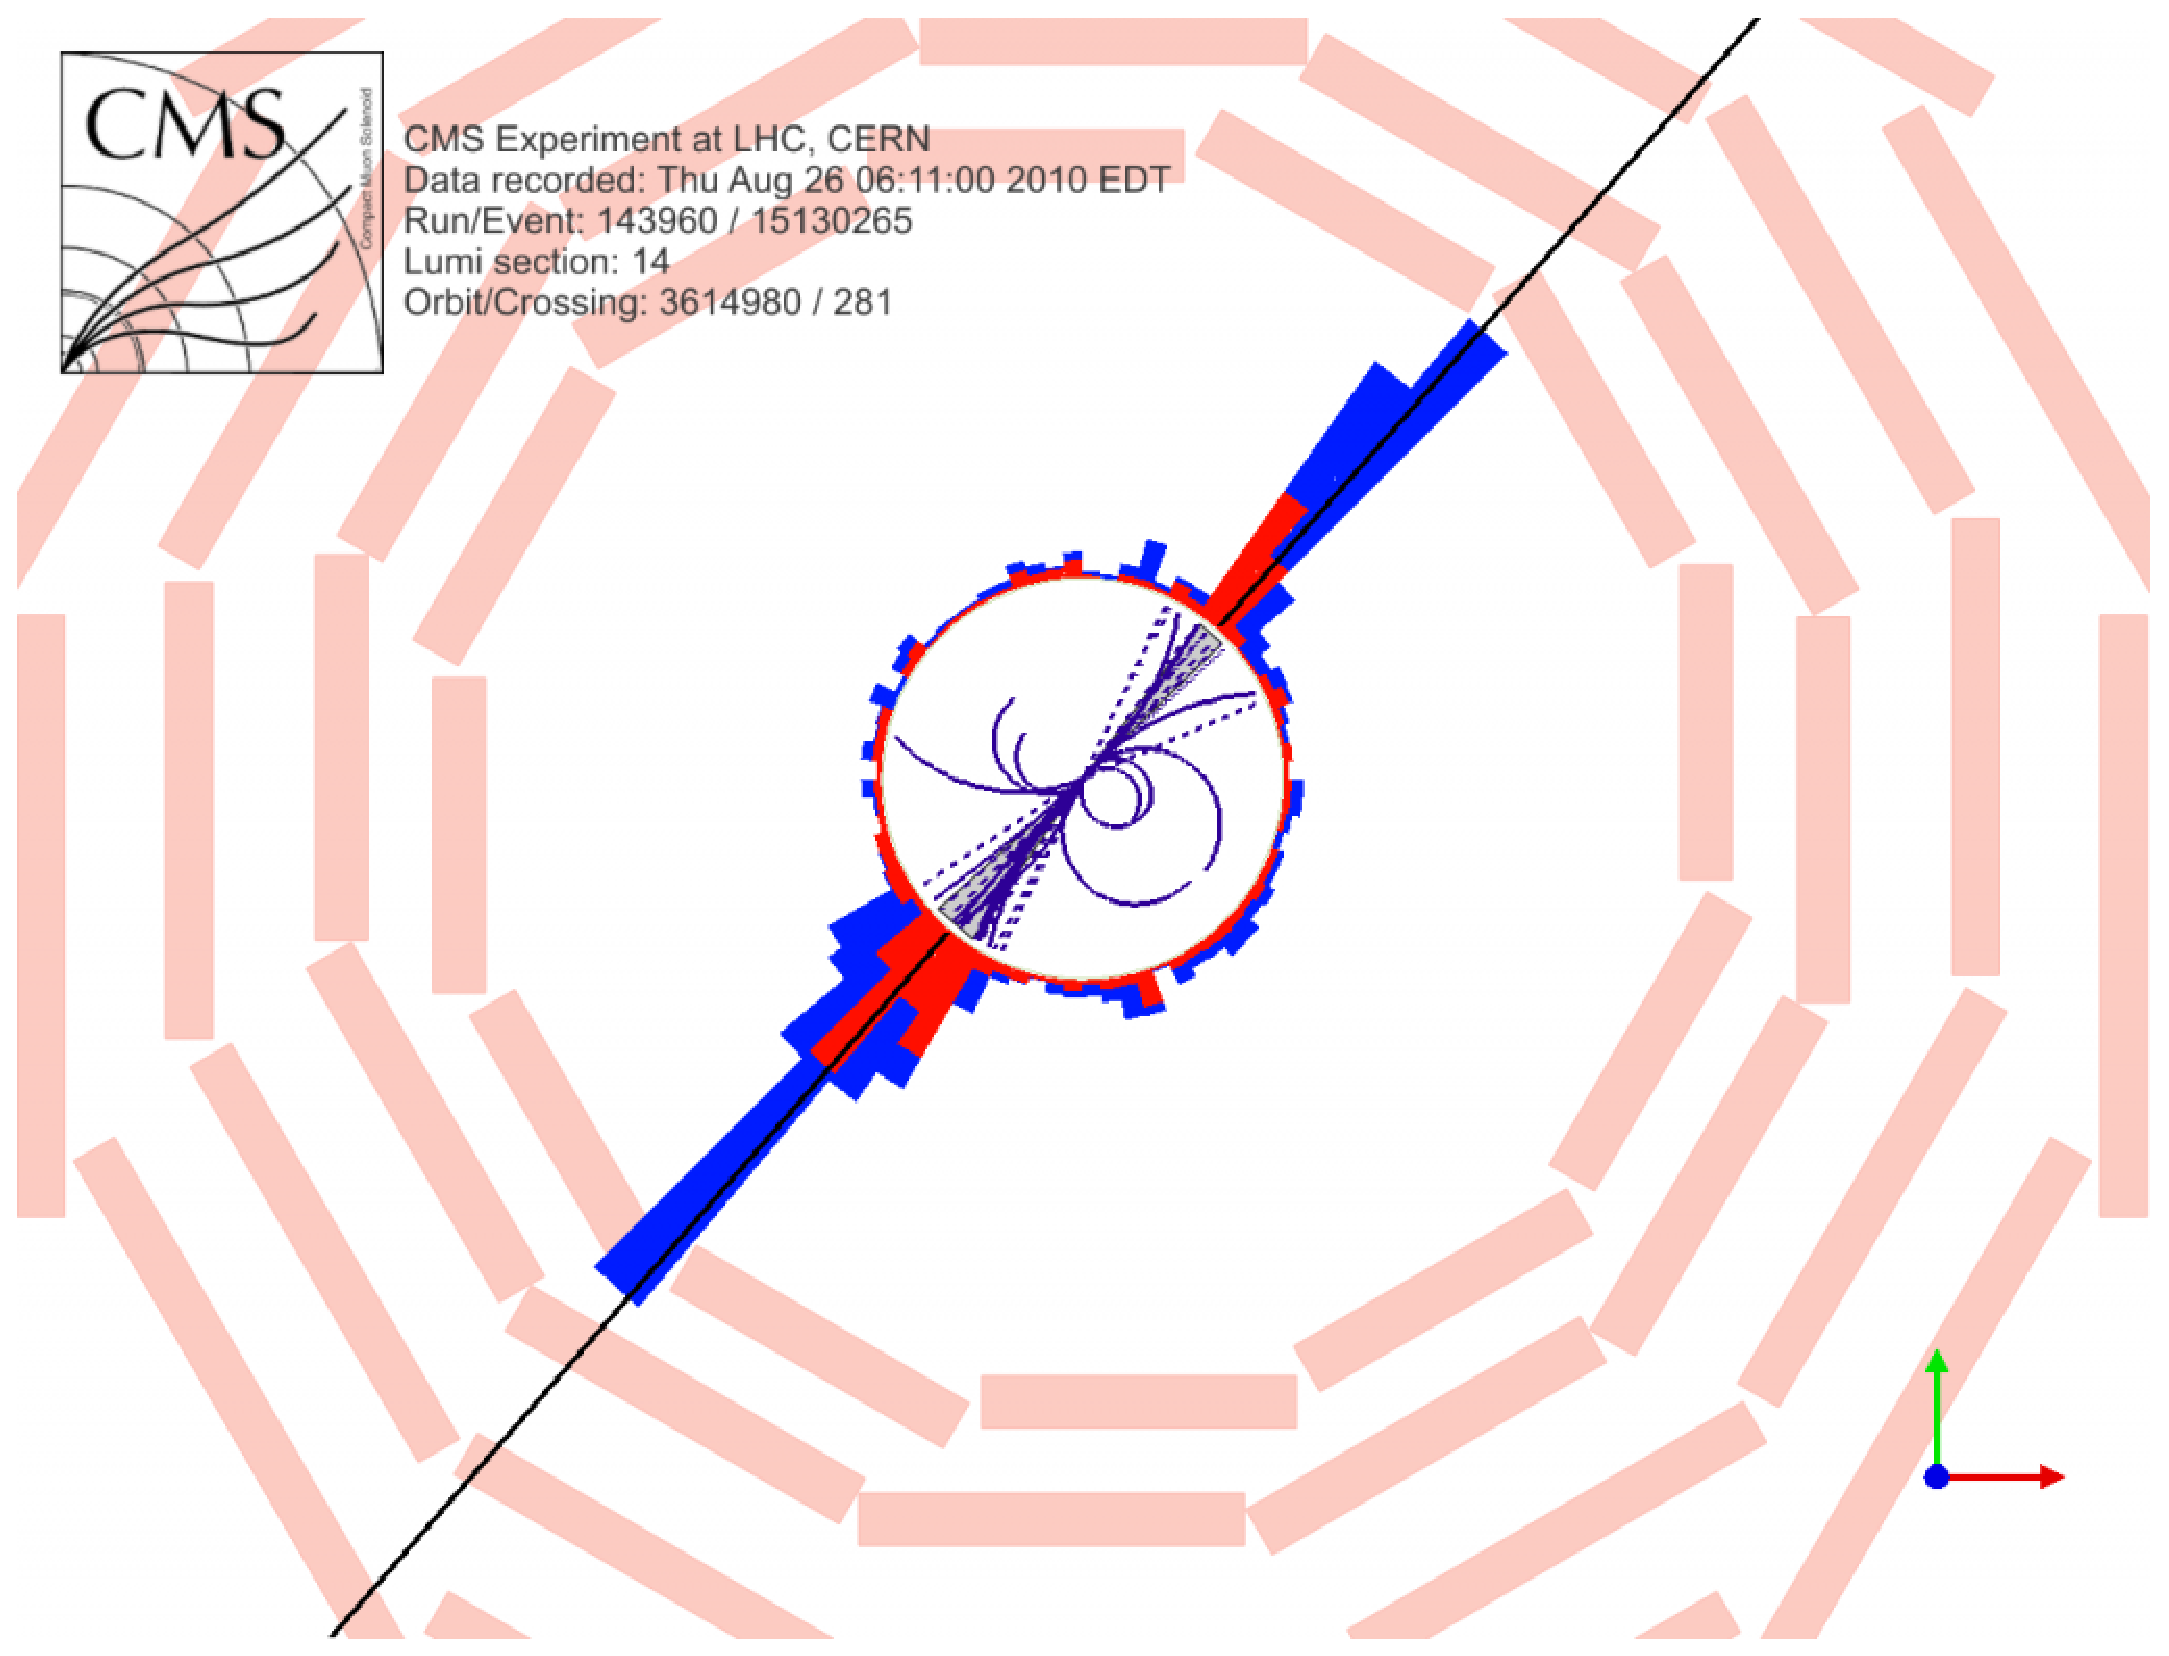
\includegraphics[width=.6\textwidth]{dijet}
    \end{figure}
\end{frame}

\begin{frame}
    \frametitle{Signal vs background}
    \begin{figure}[h]
        \centering
            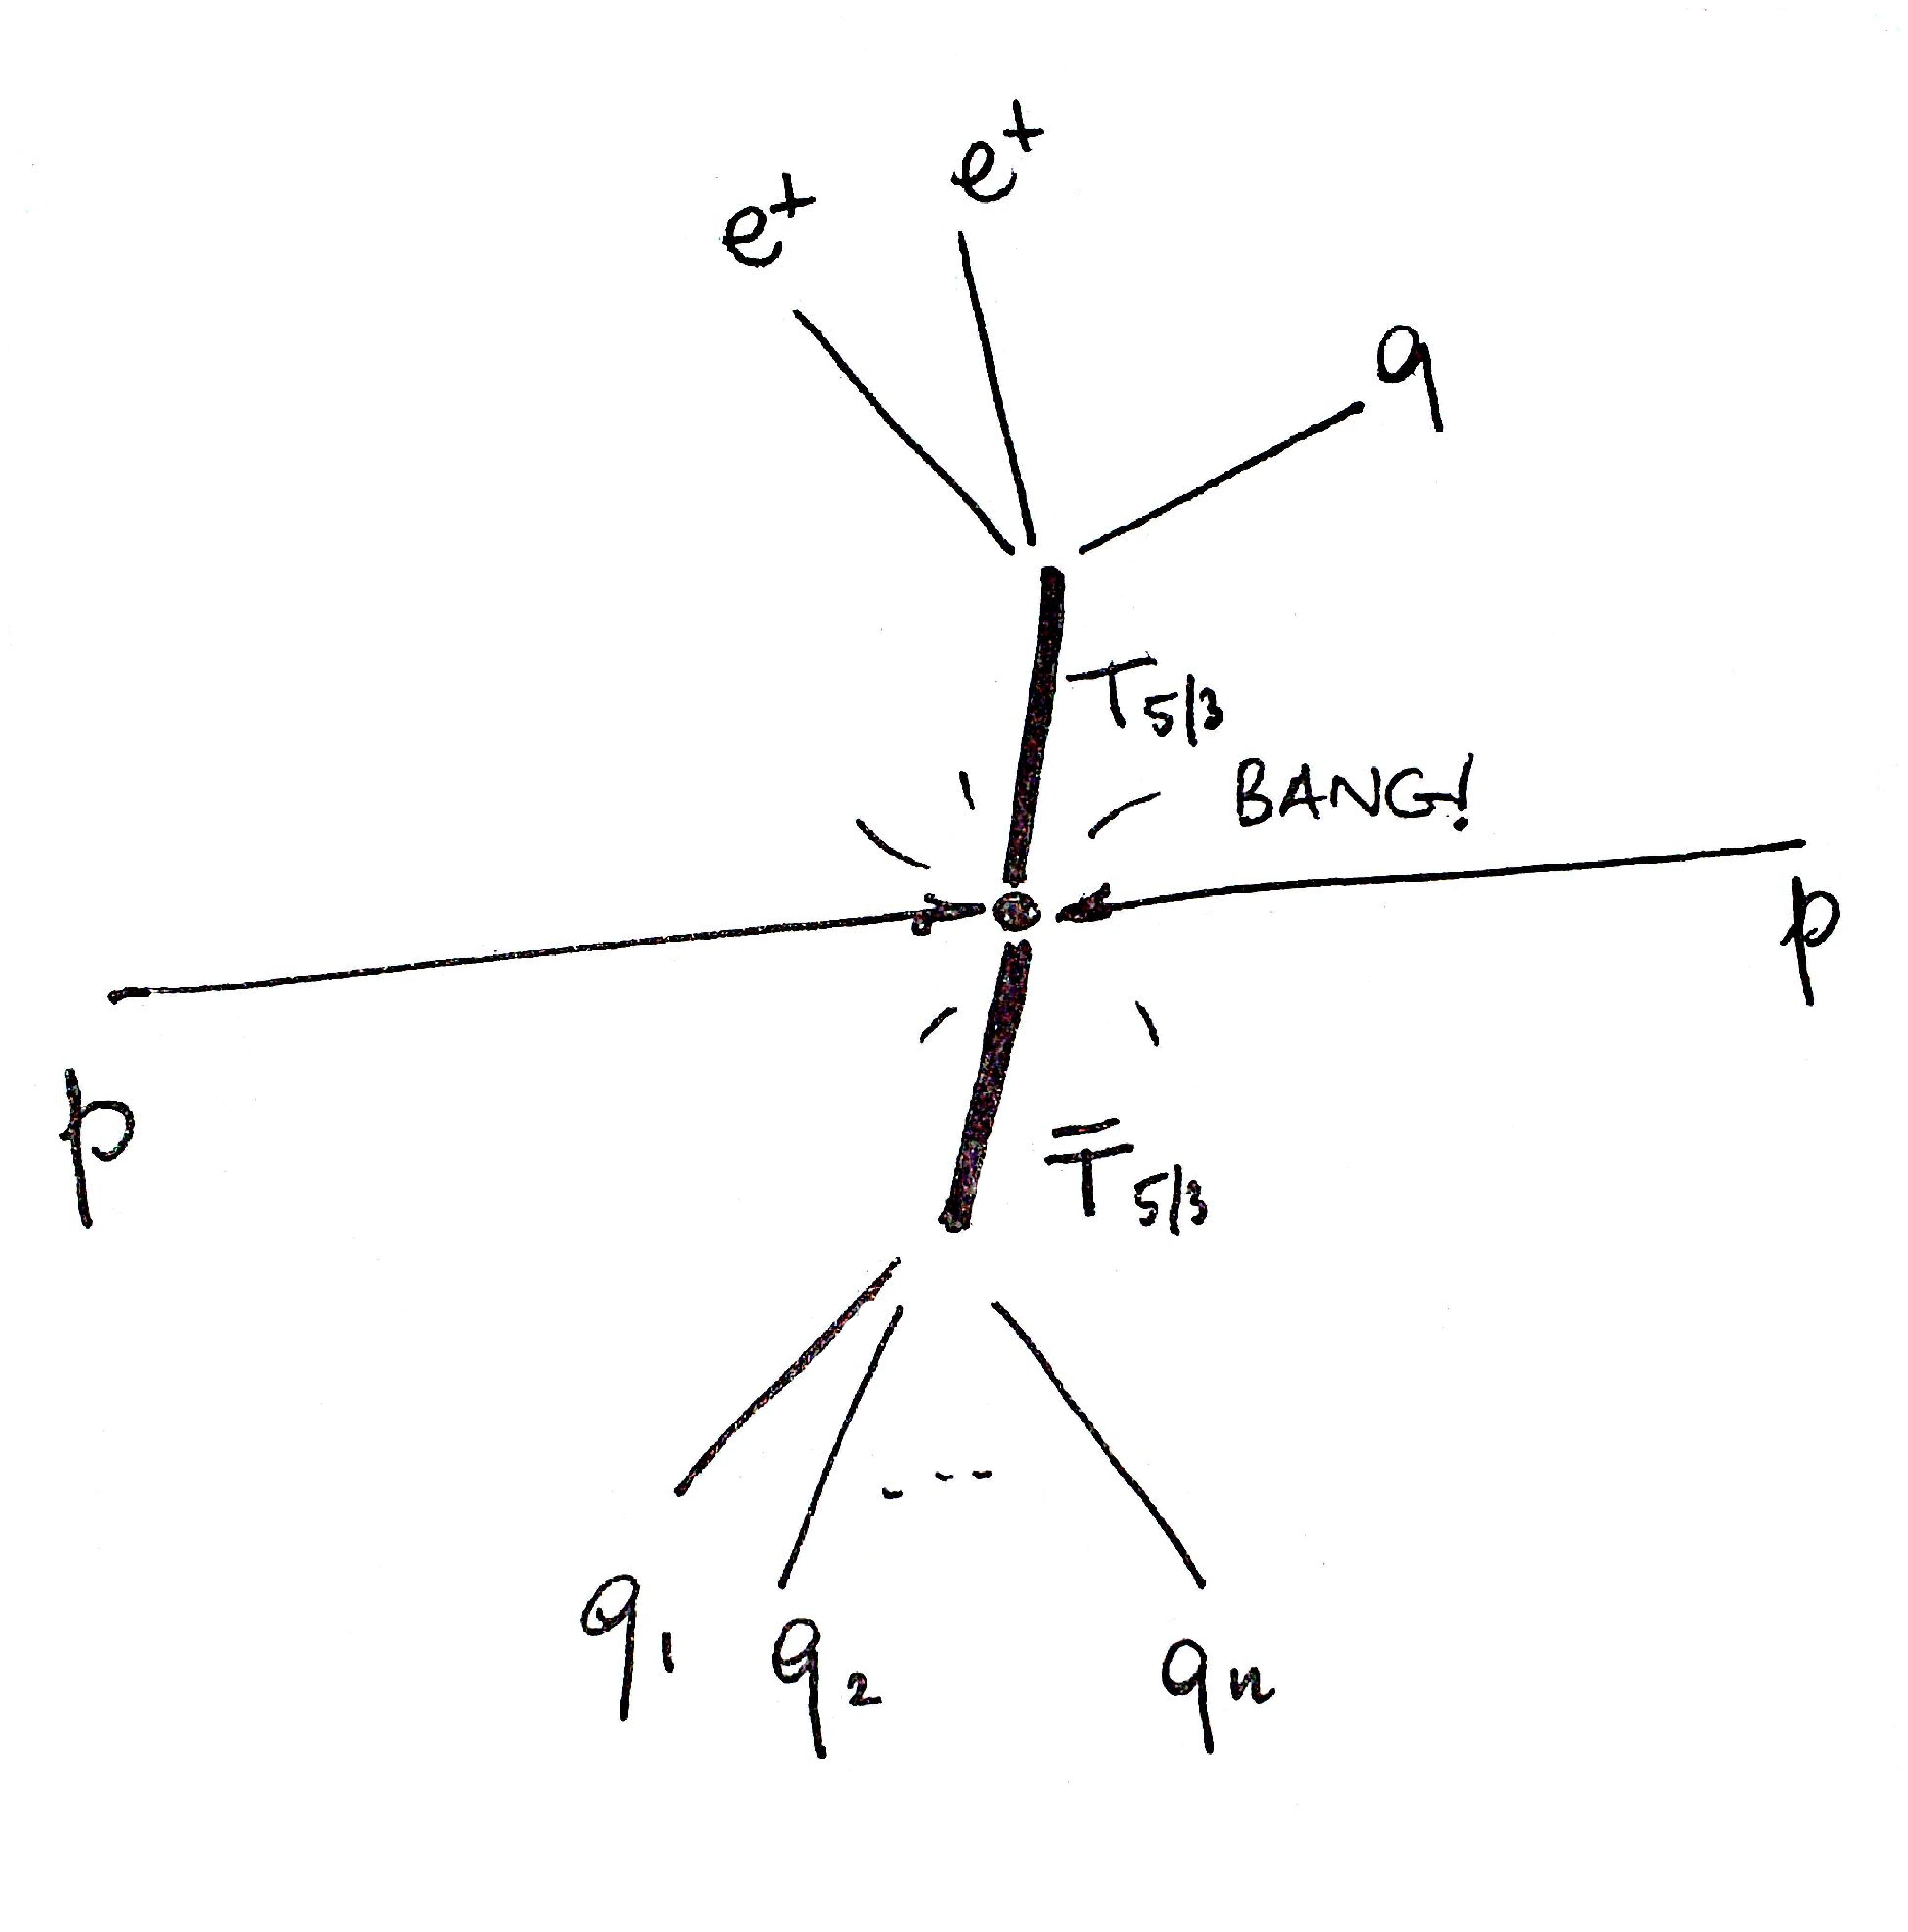
\includegraphics[width=.4\textwidth]{toppartner_decay}
    \end{figure}
    \begin{description}
        \item[True background:] other Standard Model particles decaying in
            the same way.
        \item[Fake background:] charge misidentification, leptons coming
            from secondary decays.
    \end{description}
\end{frame}

\begin{frame}
    \frametitle{The data analysis}
    Signal is extremely small! A handful of events out 
    of 40 trillions of collisions.
    \begin{block}
        {Selections}
        Find the best variables for signal/background discrimination.\\
        Careful checks with Monte Carlo simulations.
    \end{block}
\end{frame}

\begin{frame}
    \frametitle{Example: $H_T$}
    \framesubtitle{The momentum of the jets in the event, in a plane
    perpendicular to the beam line.}
    \begin{figure}[h]
        \centering
            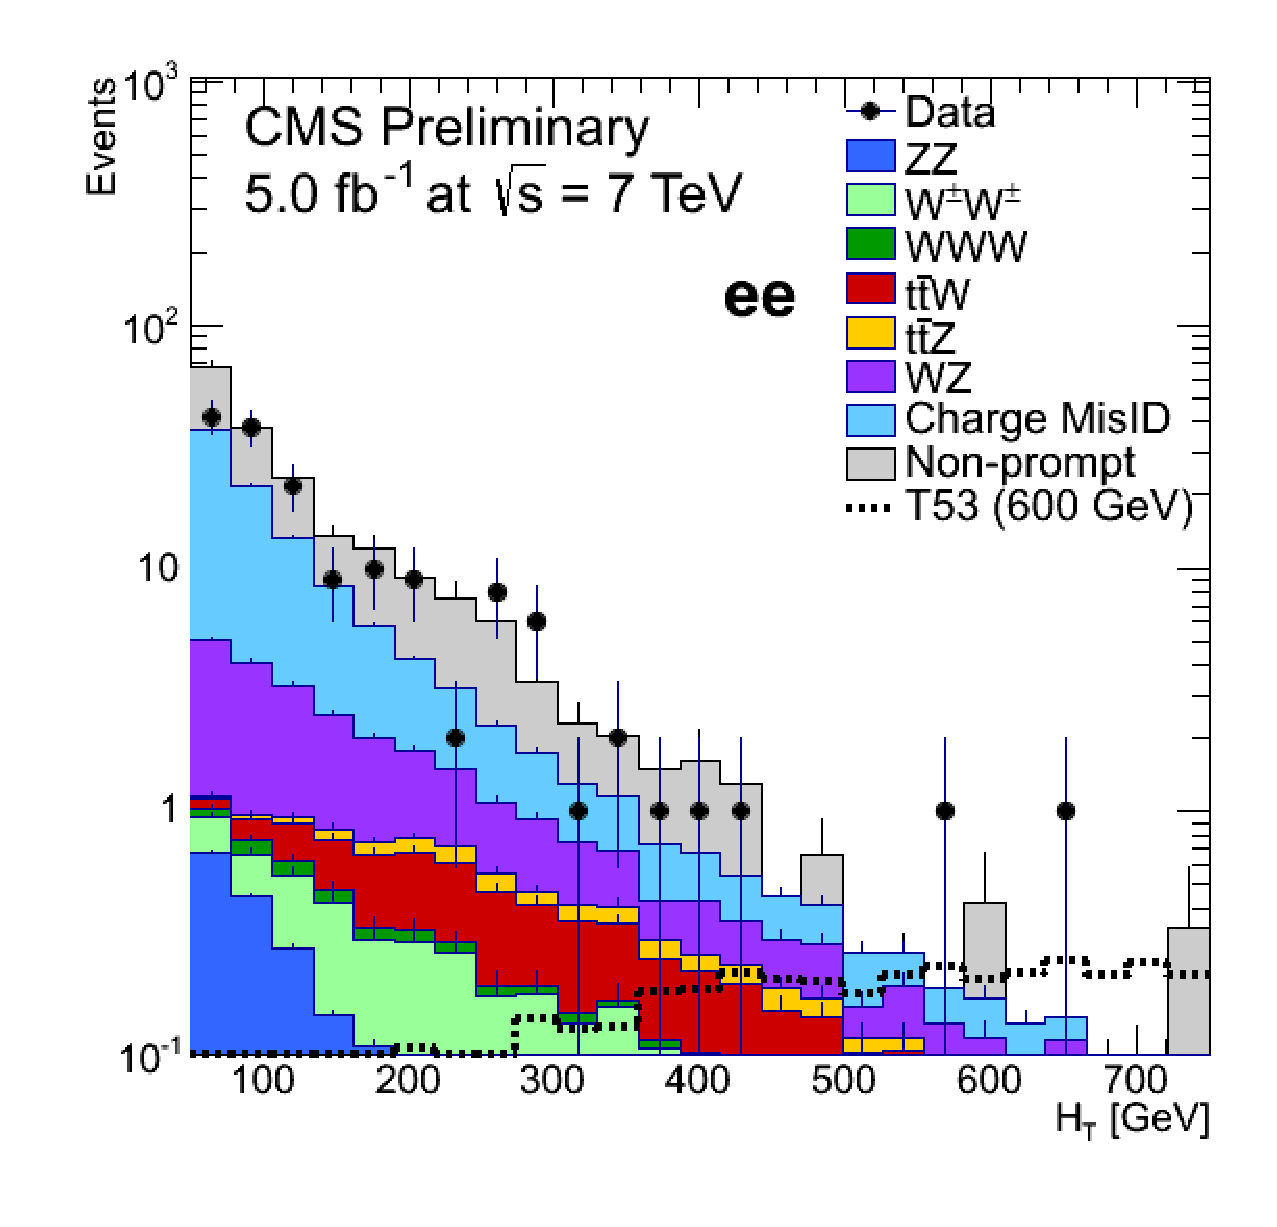
\includegraphics[width=0.4\textwidth]{ht}
    \end{figure}
\end{frame}

\begin{frame}
    \frametitle{Do the top partners exist?}
    \begin{figure}[h]
        \centering
            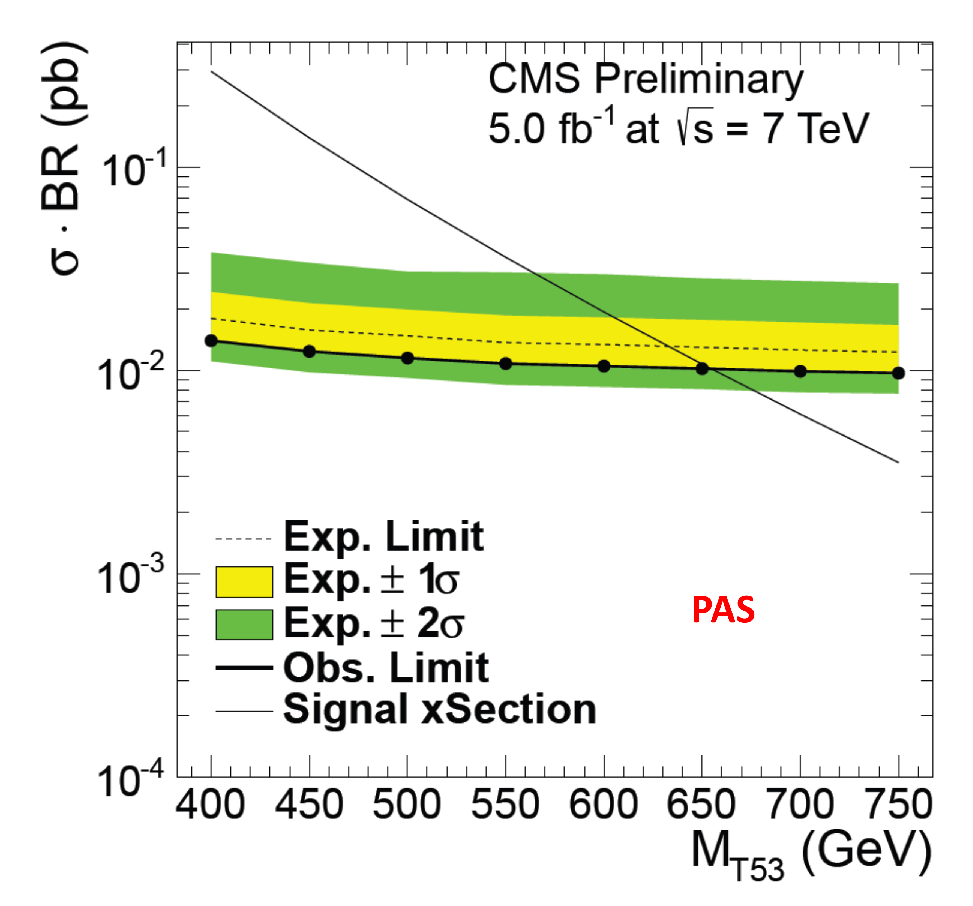
\includegraphics[width=0.4\textwidth]{limit}
    \end{figure}
    Excluded at 95\% CL for masses below \unit[655]{GeV/$c^2}$.
\end{frame}

\end{document}
